%%%%
%%%% Main Matter
%%%%

\addstarredpart{Part Zero}

\cleardoublepage
\chapter*{Table des matières}
\parttoc


\chapter[Introduction]{Introduction}

Ce chapitre présente brièvement les deux principaux objets étudiés pendant cette thèse~: les algorithmes
de chiffrement par bloc et les fonctions de hachage cryptographiques. Il est une traduction
des deux premiers chapitres de la première partie de ce manuscrit.

\medskip

\begin{center}
\aldineleft
\end{center}

\medskip


\section{Algorithmes de chiffrement par bloc}

Un \emph{algorithme de chiffrement par bloc} (ou chiffrement (par bloc), ou chiffre (par bloc)) est une famille d'applications
injectives de domaine et codomaine finis. On adoptera en fait toujours ici une vision plus spécifique de ces objets,
considérant des domaines et codomaines de même taille, et tous les paramètres impliqués étant définis sur un alphabet
binaire. Ainsi, on considère qu'un chiffre par bloc est une application
$\E : \{0,1\}^\kappa \times \{0,1\}^n \rightarrow \{0,1\}^n$
telle que pour tout $k \in \{0,1\}^\kappa$, $\E(k,\cdot)$ est une permutation.
On appelle
$\kappa$ la \emph{taille de clef} et $n$ la \emph{taille de bloc} de $\E$. Habituellement, ces paramètres ont pour valeur
$\kappa \in \{64, 80, 128, 192, 256\}$, bien que les clefs de 64 ou 80 bits ne soient plus considérées de nos jours
comme apportant une sécurité suffisante, et 
$n \in \{64, 128, 256\}$.
On requiert aussi que $\E$ est son inverse $\E^{-1}$ soient calculables efficacement (bien qu'en fonction des applications
il puisse être suffisant qu'un seul des deux le soit). 

L'emploi le plus direct d'un chiffre par bloc est de permettre d'assurer la confidentialité de communications.
Deux partis $A$ et $B$ partageant une clef $k$ pour le même chiffre\footnote{Nous ne nous intéresserons pas ici à la question de savoir
comment obtenir un tel partage.} peuvent communiquer par l'intermédiaire de messages chiffrés $c \defas \E(k,p)$,
$c' \defas \E(k,p')$, etc. Le second argument $p$ de $\E$ est généralement appelé 
\emph{texte clair}, et le résultat $c$ est généralement appelé \emph{texte chiffré}.

Si $\E$ est tel que la permutation $\E(k,\cdot)$ est difficile à inverser quand $k$ est inconnu, $A$ et $B$
pourraient s'attendre à ce qu'un canal de communication sûr consiste à injecter leurs messages
vers les chaînes
$m_0||m_1||\ldots||m_\ell$ de tailles multiples de $n$ et envoyer les chiffrés
$\E(k,m_0)||\E(k,m_1)||\ldots||\E(k,m_\ell)$.
Ce schéma comporte cependant deux problèmes de taille, indépendamment de la sécurité du chiffrement choisi~:
en premier lieu, le schéma est déterministe, c'est à dire que chiffrer le même texte clair plusieurs fois résulte toujours en le
même chiffré. Un adversaire passif espionnant la conversation sur le canal entre $A$ et $B$ peut donc
détecter quand deux messages identiques ont été envoyés. En second lieu, la communication n'est pas authentifiée. Un
adversaire actif présent sur le canal peut supprimer et modifier certains des blocs d'un message,
ajouter des blocs d'un précédent message, ou encore ajouter des blocs générés aléatoirement. Tout ceci peut
être fait sans que $A$ et $B$ ne détectent qu'un autre parti agit sur le canal avec des intentions hostiles. 

Des problèmes tels que ceux ci-dessus sont résolus en concevant des \emph{modes d'opération} sûrs. Nous n'étudions
pas ceux-ci dans ce manuscrit, mais mentionnons tout de même certains éléments qui leur sont liés dans
la section \ref{sec:cf_modes}. Dans l'immédiat, nous nous consacrons à rendre l'intuition derrière les critères de sécurité
d'un chiffre par bloc plus explicites. 

\subsection{Sécurité des chiffres par bloc}

Comme le reste de cette introduction, cette section est relativement informelle. Notre but est d'expliquer en
quoi consiste un bon chiffre par bloc, d'un point de vue pratique. Nous commençons toutefois par d'abord
définir une idéalisation de cette primitive, sous la forme du modèle du \emph{chiffre idéal}.

\begin{fdefi}[Chiffre par bloc idéal]
Un \emph{chiffre par bloc idéal} $\E$ est une application
$\{0,1\}^\kappa \times \{0,1\}^n \rightarrow \{0,1\}^n$ telle que toutes les permutations
$\E(k,\cdot)$ sont tirées aléatoirement et uniformément parmi les permutations de $\{0,1\}^n$.
\end{fdefi}

Cette notion correspond intuitivement à ce qu'on peut atteindre de mieux étant donnée la définition d'un chiffre par bloc.
Pour de petites valeurs de $n$ (par exemple jusqu'à $20 \sim 32$ en fonction de la performance souhaitée), on peut
implémenter un chiffre idéal en utilisant un algorithme de mélange approprié, par exemple celui attribué de façon
variable à Fisher, Yates, Knuth, etc.~\cite{uniform_shuffle}, que nous appellerons «\,FYK\,».
Avec cette méthode, calculer la permutation associée à une certaine clef fixe a une complexité de
$\bigo(2^n)$ en temps et en mémoire, ce qui n'est
évidemment pas satisfaisant pour les tailles classiques de blocs $n \geq 64$ utilisées en cryptographie.
Même pour de petites valeurs de $n$, utiliser FYK requiert une quantité considérable d'aléa paramétrisé par une clef,
ce qui n'est pas quelque chose d'évident à obtenir. 
Tout ceci fait qu'en pratique nous sommes généralement forcés d'utiliser des «\,approximations\,» de chiffres idéaux.
Une façon utile, bien qu'essentiellement théorique, de quantifier la sécurité d'un chiffre par bloc est alors précisément
de mesurer à quel point celui-ci est éloigné d'un chiffre idéal.
Informellement, ceci est fait en bornant par le haut l'\emph{avantage} sur un choix aléatoire qu'un adversaire
avec des ressources bornées de façon appropriée a de distinguer s'il interagi avec une permutation tirée aléatoirement
ou avec une instance du chiffre paramétré avec une clef aléatoire (et inconnue). Cette proposition peut être précisée
sous la forme suivante, similaire à celle qui peut être trouvée par exemple dans~\cite{DBLP:journals/jcss/BellareKR00}~:

\begin{fdefi}[Permutations pseudo-aléatoires (PRP)]
Soit $\E$ un chiffre par bloc de taille de clef $\kappa$ et de taille de bloc $n$.
On note 
$\Pi_{2^n}$ l'ensemble des permutations sur les chaînes binaires de longueur $n$~; $x \overset{\$}{\leftarrow} \mathcal{S}$
l'action de tirer $x$ aléatoirement et uniformément parmi les éléments de l'ensemble $\mathcal{S}$~; $\mathcal{A}^{f}$
un algorithme ayant accès à un oracle $f$ et qui retourne un unique bit.
On définit alors 
l' \emph{avantage PRP} de $\mathcal{A}$ pour $\E$, écrit $\Adv^{\text{PRP}}_{\E}(\mathcal{A})$ comme~:
\[
\Adv^{\text{PRP}}_{\E}(\mathcal{A}) = |\Pr[\mathcal{A}^f = 1~|~f \overset{\$}{\leftarrow} \Pi_{2^n}] - \Pr[\mathcal{A}^f = 1~|~f \defas \E(k,\cdot), k \overset{\$}{\leftarrow} \{0,1\}^\kappa]|.
\]
La \emph{sécurité PRP} de $\E$ pour une \emph{complexité en donnée} $q$ et une \emph{complexité en temps} $t$ est~:
\[
\Adv^{\text{PRP}}_{\E}(q,t) \defas \max_{\mathcal{A}\,\in\,\text{Alg}^{f\backslash q, \E\backslash t}} \{\Adv^{\text{PRP}}_{\E}(\mathcal{A})\}.
\]
Ici, 
$\text{Alg}^{f\backslash q, \E\backslash t}$ est l'ensemble des algorithmes $\mathcal{A}$ qui ont accès à un oracle $f$ auquel ils font au plus $q$ accès,
et qui tournent en temps inférieur à
$\bigo(t)$, l'unité de temps étant le temps nécessaire pour calculer $\E$ une fois.
\label{def:fprp}
\end{fdefi}
Il existe également une notion similaire de \emph{permutation fortement pseudo-aléatoire} (SPRP) qui considère des algorithmes ayant accès à la fois à l'oracle $f$ et à son inverse.

\medskip


La notion de PRP est utile dans certains contextes, par exemple pour prouver qu'une construction utilisant un chiffre par bloc n'est pas significativement moins
sûre que ce dernier. Un tel résultat est typiquement obtenu en définissant une fonction d'avantage pour la construction de haut niveau
similaire à celle utilisée dans la sécurité PRP, et en montrant
que cet avantage n'est pas plus qu'une fonction «\,raisonnable\,» de la sécurité PRP.
Par exemple, dans le cas de \cite{DBLP:journals/jcss/BellareKR00}, la construction de haut niveau considérée est CBC-MAC.

Toutefois, la définition~\ref{def:fprp} n'est pas constructive, dans le sens où elle ne donne pas de procédure efficace permettant de calculer la sécurité PRP
d'un chiffre par bloc en général, bien que certains résultats existent pour des constructions spécifiques, qui nécessitent alors généralement l'accès à une
primitive idéale de bas niveau comme une «\,permutation aléatoire\,».
Un des objectifs majeurs de la cryptographie symétrique consiste à analyser explicitement des instances de chiffres par blocs dans le but d'établir leur sécurité
concrète contre certaines attaques. S'inspirant de la terminologie de la définition~\ref{def:fprp}, ceci revient à trouver
des algorithmes pour lesquels $q$, $t$ et l'avantage PRP sont connus. Une telle attaque sur un chiffre $\E$ permet alors de borner par le bas sa sécurité PRP
en un certain point.
Cependant, en réalité, le monde de la cryptanalyse des chiffres par bloc est plus nuancé que ce que la définition~\ref{def:fprp} pourrait nous faire croire.
Des caractéristiques importantes d'une attaque sont aussi sa complexité en mémoire~; la quantité de calculs qui ont lieu en ligne ou hors ligne~; savoir si elle s'applique
aussi bien à toutes les clefs ou à seulement certaines d'entre elles~; savoir si elle permet de retrouver $k$ quand $f$ est une instance de $\E$, ou un algorithme
équivalent à $\E(k,\cdot)$, etc.
Nous consacrons le reste de cette section à introduire quelques éléments typiques de telles attaques concrètes sur des chiffres par bloc.

\subsection{Distingueurs et attaques}

L'essence de beaucoup d'attaques concrètes sur les chiffres par blocs est faite de \emph{distingueurs}, qui peuvent être définis comme des algorithmes utilisant des ressources
raisonnables qui ont un avantage non négligeable d'après la définition~\ref{def:fprp}.
Il n'existe pas de réponse évidente à ce que «\,raisonnable\,» et «\,non négligeable\,» signifient dans le contexte d'attaques réelles, notamment parce que les tailles de clefs
et de blocs sont fixes. Si certains chiffres ou distingueurs potentiels peuvent être paramétrés pour aider à donner du sens à cette définition, ce n'est pas toujours le cas.
On peut aussi parfois être facilement convaincu par la performance d'un algorithme, et il n'y a alors pas de doutes sur le fait qu'il constitue en un distingueur
(par exemple distinguer $\E$ de clef et bloc de taille 128 avec $q = 2$, $t = 2^{20}$, probabilité $\approx 1$), tandis que dans d'autres cas la situation est bien
moins claire (par exemple $q = t = 2^{120}$ et probabilité $\approx 1$). Nous ignorons entièrement ces problèmes potentiels dans le reste de cette introduction et considérons
que toutes les attaques mentionnées sont consensuelles.

\subsubsection{Classes de distingueurs}

Nous décrivons brièvement deux types de distingueurs qui exploitent des comportements non idéaux de différentes natures.

\bigskip

Nous commençons par présenter les \emph{distingueurs différentiels}, qui font partie de la classe plus générale des distingueurs
dits \emph{statistiques}.
L'idée de base correspondant à cette dernière est de définir un événement dont la distribution de probabilité pour sa cible
(le chiffre par bloc $\E$) est différente de celle obtenue pour une permutation tirée aléatoirement dans $\Pi_{2^n}$.
Appliquer le distingueur correspond alors à collecter un certain nombre d'échantillons (obtenus grâce à un oracle)
et à déterminer quelle est la distribution d'après laquelle ils ont le plus probablement été tirés.
Un distingueur différentiel réalise cette idée en considérant un certain type d'événement statistique. Une autre classe
majeure de distingueurs statistique est celle des \emph{distingueurs linéaires}.

Soit $\E$ un chiffre par bloc, une \emph{différentielle} pour $\E$ est une paire
$(\Delta,\delta)$ de différences d'entrée et de sortie associées à une certaine loi de groupe
$+$\footnote{On considérera toujours des différences non triviales avec $\Delta \neq 0$.}.
Dans la grande majorité des cas, $+$ est l'addition sur $\mathbf{F}_2^n$,
c'est à dire le OU exclusif bit à bit (XOR)~; on utilisera alors souvent la notation alternative $\oplus$ pour cette loi.
Parfois, $+$ est l'addition dans $\mathbf{Z}/2^n\mathbf{Z}$, et d'autres fois les différences peuvent être considérées suivant plusieurs lois à la fois.
Une \emph{paire différentielle} pour la différence $(\Delta,\delta)$ et pour une certaine clef $k$
est une paire ordonnée de textes clairs et de leurs chiffrés correspondant $\langle (p,c), (p',c')\rangle$ avec 
$p$, $c \defas \E(k,p)$, $p'$, $c' \defas \E(k,p')$, telle que $p - p' = \Delta$, $c - c' = \delta$. Quand la différence est sur $\mathbf{F}_2^n$,
la soustraction coïncide avec l'addition et la paire peut être non ordonnée. Nous nous plaçons dans un tel cas pour le reste de cette description.

On appelle \emph{probabilité différentielle} d'une différentielle pour une permutation $\Perm$ la probabilité d'obtenir une
paire différentielle pour $\Perm$~:
$\DP^{\Perm}(\Delta,\delta) \defas \Pr_{p\,\in\,\{0,1\}^n}[\Perm(k,p) \oplus \Perm(k,p \oplus \Delta) = \delta]$.
La caractéristique la plus importante d'une différentielle pour un chiffre par bloc est sa \emph{probabilité différentielle attendue},
qui est simplement la moyenne sur $k$ de ses probabilités différentielles pour $\E(k,\cdot)$~:
$\EDP^{\E}(\Delta,\delta) \defas 2^{-\kappa}\sum_{k\,\in\,\{0,1\}^\kappa} \DP^{\E(k,\cdot)}(\Delta,\delta)$.
Une hypothèse courante est que pour la plupart des clefs et des différentielles, la probabilité DP à clef fixée
est proche de la moyenne EDP.
La DP d'une différentielle aléatoire pour une permutation aléatoire peut être approchée par une loi de Poisson~:
le nombre (approché) de paires différentielles est
$\sim \poi(2^{-1})$, de moyenne et variance $2^{-1}$
(voir~\cite{DBLP:journals/jmc/DaemenR07}, se basant sur un résultat antérieur~\cite{DBLP:journals/joc/OConnor95}).
Puisqu'il y a
$2^{n-1}$ paires possibles, la DP attendue est de $2^{-n}$\footnote{On notera cependant que la DP prend forcément sa valeur parmi les multiples de $2^{-n+1}$.}.
Pour qu'un distingueur sur $\E$ soit utile, il faut donc en quelque sorte que son EDP soit différente de $2^{-n}$. Si elle en est suffisamment éloignée
(par exemple $2^{-3n/4}$), on fait généralement l'hypothèse simplificatrice que toutes les DPs sont égales à leur espérance (ou plutôt la valeur
possible la plus proche).
Dans ce cas,
utiliser un distingueur consiste à accumuler
$\propto 1/\EDP^{\E}(\Delta,\delta)$ textes clairs vérifiant la différence d'entrée et à compter combien d'entre eux vérifient la différence de sortie.
Le distingueur fait l'hypothèse qu'il
interagit avec $\E$ si et seulement si cette valeur est au moins un.

\bigskip

Tous les distingueurs ne sont pas statistiques;
un autre type de distingueur est basé sur une représentation \emph{algébrique} des chiffres par bloc.
Il est toujours possible de redéfinir un chiffre 
$\E : \{0,1\}^\kappa \times \{0,1\}^n \rightarrow \{0,1\}^n$ comme un ensemble ordonné de fonctions $\F_i : \{0,1\}^{\kappa+n} \rightarrow \{0,1\}$ projetant
$\E$ sur son $i^\text{ème}$ bit de sortie~: $\E \equiv \langle \F_0, \ldots, \F_{n-1} \rangle$. Les $\F_i$s peuvent être vues comme des fonctions booléennes
$\mathbf{F}_{2^{\kappa + n}} \rightarrow \Ftwo$ qui sont elles mêmes en bijection avec les éléments de $\Ftwo[x_0,x_1,\ldots x_{\kappa + n-1}]/<x_i^2-x_i>_{i<\kappa + n}$,
c'est à dire des polynômes en $\kappa + n$ variables sur $\Ftwo$. Le polynôme correspondant à une fonction booléenne est appelé sa \emph{forme algébrique normale}
(ANF)~;
l'ANF de $\E$ est l'ensemble ordonné des ANFs de ses projections.

Une caractéristique importante d'une ANF est son degré, qui peut être utilisé pour définir des distingueurs simples mais efficaces.
Le degré de l'ANF d'une permutation sur $n$ bits est au plus $n - 1$, et il est attendu d'une permutation aléatoire qu'elle soit de degré
maximal. Si un chiffre par bloc a un degré $d < n - 1$, il peut être distingué en le dérivant en suffisamment de points.
Ceci nécessite simplement d'évaluer l'oracle fourni au distingueur sur $2^d$ valeurs bien choisies (essentiellement un cube de dimension $d$) et de toutes
les additionner.
Si le résultat vaut zéro sur chaque bit, l'oracle est probablement de degré moins que $d$ et est donc supposé être $\E$~; si ce n'est pas le cas, il est
nécessairement de degré plus que $d$ et est donc supposé être une permutation aléatoire.

\subsubsection{\'Etendre un distingueur pour retrouver une clef}

Pour définir la sécurité PRP, la notion de distingueur était suffisante. Cependant, dans le cas d'attaques concrètes, l'objectif
final est idéalement de retrouver la clef inconnue utilisée par l'oracle.
Le contexte d'une attaque est aussi souvent différent de celui d'un jeu de sécurité PRP, car l'attaquant connaît généralement déjà
le chiffre $\E$ avec lequel il interagit, et sait également que celui ci n'est pas une permutation aléatoire~; il peut donc paraître finalement inutile
d'appliquer un distingueur.
Malgré ces observations, les distingueurs sont utiles dans bien des cas, et sont souvent à la base d'attaques retrouvant la clef\footnote{Toutes ces
attaques ne sont pas pour autant basées sur des distingueurs. Bien que beaucoup d'entre elles soient intéressantes, nous ne les décrivons pas ici.}.
Nous expliquons maintenant brièvement l'idée derrière ces conversions de distingueurs en attaques plus complètes. Pour ceci, nous devons faire
certaines hypothèses sur la structure de $\E$, toujours valables en pratique.

Un  \emph{chiffre par bloc itératif} est un chiffre $\E$ pouvant être décrit comme la composition multiple
d'une \emph{fonction de tour} $\R$, possiblement aussi composée avec une fonction d'initialisation et une fonction de finalisation
que nous ignorons ici~:
$\E \equiv \R \circ \cdots \circ \R$. On note $r$ le nombre total d'applications de $\R$ dans $\E$ pour une version «\,complète\,» de ce dernier.
Une attaque basée sur un distingueur et dont l'objectif est de recouvrir la clef consiste tout d'abord à trouver un distingueur sur une version
réduite de $\E$ constituée de la composition de $d < r$ fonctions de tour. L'étape suivante consiste alors à interroger l'oracle sur
des entrées vérifiant les conditions du distingueur (par exemple des textes clairs de différence $\Delta$)~; les réponses obtenues étant chiffrées
avec une version complète du chiffrement, il n'est pas attendu du distingueur qu'il réussisse avec un avantage non négligeable.
Cependant, l'idée principale de l'attaque (et la dernière étape) consiste à faire
une hypothèse sur la valeur d'une partie de la clef inconnue $k$ de $\E$,
qui lui permet de déchiffrer partiellement les textes chiffrés sur $r-d$ tours. Ainsi, si l'hypothèse était correcte, l'attaquant obtient des chiffrés pour le
chiffre réduit à $d$ tours, pour lequel l'avantage du distingueur est supposé non négligeable.
En revanche, si l'hypothèse est fausse,
il obtient des chiffrés équivalents à ceux d'un chiffre sur $2r - d$ tours, et le distingueur aura probablement à nouveau un avantage négligeable.
Finalement, on peut donc
voir que cette approche donne une méthode pour vérifier une hypothèse sur une partie a priori inconnue de la clef.

On peut faire certains commentaires concernant cette procédure. Tout d'abord, le coût associé aux hypothèses répétées sur la valeur d'une partie de la clef
font évidemment que la complexité de l'attaque sera supérieure à celle du distingueur. On ne peut donc utiliser de cette façon que
des distingueurs de complexité suffisamment faible.
Ensuite, il peut y avoir plusieurs raisons faisant qu'un distingueur a priori défini sur l'ensemble d'un
chiffre $\E$ reste exploitable même si par hypothèse seulement une partie de la clef est connue, par exemple
parce que seulement une partie de la clef est utilisée chaque tour, ou parce que le distingueur ne base sa réponse que sur une partie de l'«\,état\,» du chiffre.
Enfin, la partie de la clef qui n'est pas retrouvée grâce au distingueur peut être déterminée de plusieurs façons~; par exemple, un autre distingueur
impliquant une hypothèse sur une autre partie de la clef peut être utilisé, ou alors elle peut simplement être énumérée exhaustivement.


\subsubsection{Modèles d'attaques}

Jusqu'à présent, nous avons considéré la sécurité des chiffrements dans un cas simple où l'attaquant a accès à un unique oracle secret.
Ce scénario peut être généralisé de plusieurs façons, par exemple en donnant accès à plus d'un oracle. Une généralisation de ce type qui est
relativement courante consiste en le modèle d'attaques à \emph{clefs liées}, où l'attaquant peut appeler
$\E(k,\cdot)$, $\E(\rka(k),\cdot)$, avec $\rka(\cdot)$ une ou plusieurs applications sur l'espace de clefs.
Une observation cruciale est que dans ce cas $\rka$ ne peut pas être arbitraire, car certaines applications sont suffisamment puissantes
pour permettre d'attaquer n'importe quel chiffre~; il ne peut alors pas y avoir de définition sensée de la sécurité de $\E$ dans un tel cas.
Il est donc utile de garder à l'esprit qu'une attaque doit toujours être spécifiée dans un modèle clair. Bien que certains modèles puissent
être considérés comme peu réalistes et donc peu utiles (ce qui est une critique souvent formulée à l'égard des attaques en clef liée), cette
question est toujours secondaire par rapport à celle de savoir si un modèle permet de mener des attaques triviales dans n'importe quelle circonstance. 

\subsection{Utiliser des chiffres par bloc}
\label{sec:cf_modes}

Nous avons mentionné au début de ce chapitre qu'un chiffre par bloc n'offre pas nécessairement une sécurité suffisante s'il est mal employé.
On appelle \emph{mode d'opération} une construction à base d'une primitive telle qu'un chiffre par bloc, résultant en un cryptosystème (qu'on espère) fonctionnel.
Nous ne décrivons pas de mode dans cette section, mais précisons à nouveau les critères qu'un tel objet doit vérifier.

Une condition essentielle pour un mode est qu'il doit être non déterministe, dans le sens où chiffrer le même texte clair avec la même clef deux fois ne
doit pas donner le même chiffré. Cette condition peut être formalisée par la notion d'\emph{indistinguabilité} dans un scénario d'\emph{attaque à clair choisi}
(\textsf{IND-CPA}), ainsi que ses variantes proches. Ceci est approximativement défini par le processus suivant : un adversaire est doté d'un accès
à un oracle de chiffrement pour un certain système, puis il prépare deux messages $m_0$ et $m_1$ qu'il envoie à un second oracle. Ce dernier
choisi aléatoirement un des deux messages et retourne son chiffré. Finalement, l'adversaire peut à nouveau émettre des requêtes à son premier oracle et doit ensuite
deviner quel message a été chiffré. Le cryptosystème est \textsf{IND-CPA} si aucun adversaire aux ressources bornées de façon appropriées ne réussit ce jeu
avec un avantage non marginal. Il est clair en particulier qu'aucun système déterministe ne peut être sûr suivant cette définition. 


Nous avons aussi déjà mentionné qu'un cryptosystème doit permettre aux partis communicants de s'authentifier. Ceci peut être assuré directement
par le mode d'opération (on parle alors de mode de \emph{chiffrement authentifié}), ou en combinant de façon appropriée un mode assurant le seul chiffrement avec
un \emph{code d'authentification} (MAC).
La tendance actuelle est de favoriser la première approche, qui mène généralement à des systèmes plus efficaces.


Nous concluons cette section en soulignant finalement l'importance de la \emph{borne des anniversaires} (appelée ainsi à cause du «\,paradoxe des anniversaires\,»,
que nous définissons dans la section suivante) en cryptographie en donnant la proposition suivante : la plupart des modes d'opération
utilisant un chiffre de taille de bloc $n$ ne sont sûrs que tant qu'une clef n'est pas utilisée pour chiffrer plus que $\approx 2^{n/2}$ blocs,
même si la taille de clef est largement supérieure.


%%%%%%%%%%%%%%%%%%%%%%%


\section{Fonctions de hachage}

Une fonction de hachage est une application d'un ensemble quelconque, non nécessairement fini, vers un ensemble fini de «\,petite taille\,».
Comme précédemment, nous nous restreindrons ici au cas binaire~; ainsi, on considérera qu'une  
fonction de hachage  est une application des chaînes binaires de taille arbitraire (les \emph{messages}) vers des chaînes de taille
fixe (les \emph{empreintes}, ou \emph{hachés})~:
$\hash : \{0,1\}^* \rightarrow \{0,1\}^n$ pour un entier $n$.
La plupart des fonctions de hachage ne se conforment pas strictement à cette définition et ne sont définies que sur un domaine fini, de taille par exemple égale
à $2^{64}$. Ceci n'a a priori pas d'impact en pratique, puisque les arguments potentiels d'une fonction sont bien plus petits que ces
limites supérieures, même si en toute rigueur il n'est pas évident que ceci sera toujours le cas. 
La taille de sortie typique d'une fonction de hachage est de quelques centaines de bits, et généralement un multiple de trente-deux~; des fonctions populaires
du passé et du présent peuvent être trouvées avec 
$n \in \{128, 160, 224, 256, 384, 512\}$.

Une fonction de hachage \emph{cryptographique}\footnote{Nous ne considérerons que de telles fonctions jusqu'à présent.} est une fonction
de hachage $\hash$ qui vérifie un certain nombre de \emph{propriétés de sécurité} qui expriment la difficulté de trouver des messages
produisant des empreintes vérifiant certaines conditions. On définit généralement trois propriétés «\,classiques\,» qui doivent être satisfaites
(au moins jusqu'à un certain point) par n'importe quel fonction sûre. De façon informelle, celles-ci s'expriment de la façon suivante~:

\begin{fdefi}[Résistance aux préimages]
Soit une cible $t$, un adversaire ne doit pas être capable de trouver un message
$m$ tel que $\hash(m) = t$ avec probabilité non négligeable en utilisant moins de ressources que ce qui est nécessaire pour calculer
$\hash$ $\bigo(2^n)$ fois.
\end{fdefi}
\begin{fdefi}[Résistance aux secondes préimages]
Soit un message $m$, un adversaire ne doit pas être capable de trouver un message différent $m'$ tel que
$\hash(m) = \hash(m')$  avec probabilité non négligeable en utilisant moins de ressources que
ce qui est nécessaire pour calculer $\hash$ $\bigo(2^n)$ fois.
\end{fdefi}
\begin{fdefi}[Résistance aux collisions] On ne doit pas être capable de trouver deux messages «\,frais\,» différents $m$ et $m'$ tels que $\hash(m) =
\hash(m')$ avec probabilité non négligeable en utilisant moins de ressources que ce qui est nécessaire pour calculer  $\hash$ $\bigo(2^{n/2})$ fois.
\end{fdefi}

Les complexités associées à ces définitions correspondent à celles des meilleurs algorithmes génériques connus, qui permettent de trouver
des messages avec les propriétés désirées avec forte probabilité, pour n'importe quelle fonction.
Une attaque sur une fonction de hachage concrète est un algorithme qui permet d'atteindre un des objectifs définis ci-dessus significativement
plus efficacement qu'avec le meilleur algorithme générique. Par définition, un tel algorithme viole la propriété de sécurité associée.
Dans nos définitions ci-dessus, nous mesurons la complexité des attaques en nombre d'appels à $\hash$. En pratique, il est généralement
nécessaire d'ajuster cette mesure à une granularité plus fine~; par exemple, pour une fonction de type \merkdam (que nous définissons
dans la section~\ref{sec:fmd}), il est nécessaire de mesurer cette complexité en nombre d'appels à ce qui sera défini comme
la \emph{fonction de compression}.


On peut remarquer que la cible plus basse de 
$\bigo(2^{n/2})$ pour les attaques en collision est une conséquence directe du
«\,paradoxe des anniversaires\,»~: informellement, 
$N$ éléments définissent $\bigo(N^2)$ paires~; si ces $N$ éléments sont tirés au hasard et uniformément dans un ensemble de taille $S$,
on s'attend à ce que deux d'entre eux soient les mêmes (collisionnent) avec forte probabilité après en avoir collecté
$\bigo(\sqrt{S})$. 
On peut aussi remarquer que contrairement à la résistance en (seconde) préimage, la définition de la résistance en collision n'inclus pas de «\,challenge\,» en entrée.
Ainsi, elle ne permet pas d'exclure des algorithmes (génériques) qui retournent simplement une paire de message constante qui résulte en une collision,
la complexité d'un tel algorithme étant alors indépendante de la taille de sortie $n$ de la fonction de hachage.
De tels algorithmes violent trivialement la propriété de sécurité telle qu'elle est exprimée, mais ne disent rien de pertinent sur la sécurité d'une fonction,
notamment parce qu'ils
s'appliquent aussi bien à n'importe laquelle. En conséquence, ils sont généralement entièrement ignorés dans un contexte cryptographique, et
on ne considère pas qu'ils rendent la
définition vide de sens.

\subsection{Applications des fonctions de hachage}

La nature des propriétés utilisées pour définir la sécurité d'une fonction de hachage est basée sur les contraintes imposées par les différentes utilisations qu'on peut faire
d'une telle fonction dans des cryptosystèmes ou protocoles concrets.
En fonction de la situation, la sécurité simultanée par rapport aux trois propriétés définies ci-dessus n'est pas forcément nécessaire. Par exemple, il se peut que la résistance
en collision ne soit pas nécessaire, ou que seules les attaques en seconde préimage soient une menace. Toutefois, on attend généralement d'une fonction de hachage qu'elle puisse être utilisée
dans un certain nombre de cas, et il est donc désirable qu'elle résiste à tous les types d'attaque.

Nous décrivons ci-dessous en guise d'illustration quelques utilisations possibles des fonctions de hachage.

\paragraph{Paradigme «\,hacher et signer\,».}
Une des utilisations majeure des fonctions de hachage consiste à en faire emploi dans des schémas de signature électronique.
L'objectif est de signer de longs messages efficacement et avec une bonne sécurité, étant donné un algorithme de signature
$\sign$\footnote{Nous ne définirons pas de tels algorithmes ici. Il suffit pour la compréhension de ce paragraphe
de savoir qu'ils nécessitent l'emploi d'une clef.}. En effet, directement utiliser ce dernier n'est généralement pas possible, parce qu'il est trop lent (particulièrement
comparé aux fonctions de hachage qui sont typiquement au moins $500$ à $1000$ fois plus rapide), ou aussi parce qu'il se comporte mal
pour de longs messages. Une alternative utile est alors de d'abord calculer l'empreinte du message $m$
qui doit être signé
et de ne signer que cette empreinte plutôt que le message complet.
Ceci donne des signatures de la forme $(m, \sign(k,\hash(m)))$, avec $k$ la clef utilisée pour signer avec $\sign$. 

Il est évident que pour qu'un tel schéma soit sûr, la fonction $\hash$ doit au moins être résistante en seconde préimage. Si tel n'était pas le cas, un adversaire
pourrait intercepter un message $m$ signé par $A$, remplacer $m$ par $m'$ de même empreinte, et prétendre que $A$ a signé $m'$.
Pour des raisons similaires, on peut voir que la résistance aux collisions est également nécessaire.

\paragraph{Hachage de mots de passe.} Le hachage de mots de passe est une autre application courante où une fonction
de hachage peut être utile. Dans ce cas
on suppose qu'une certaine entité souhaite autoriser des utilisateurs à s'authentifier grâce à un mot de passe.
En conséquence, elle doit mémoriser le mot de passe correspondant à chaque utilisateur. Comme il est évident que stocker les mots
de passe eux-mêmes mènerait à de grave problèmes de sécurité, une idée consiste à stocker à la place leurs images à travers une fonction
de hachage $\hash$. Ainsi, même si un adversaire devait trouver la liste des utilisateurs et de leurs mots de passe hachés associés, il ne serait
pas capable de trouver les mots de passe eux-mêmes (ou une entrée équivalente), pour peu que $\hash$ résiste aux attaques en préimage.
Dans cet exemple, résister aux attaques en seconde préimage ou en collision n'est alors pas nécessaire. Cependant, il est bon de noter
que le schéma esquissé ci-dessous est en fait trop simpliste pour apporter une réelle sécurité, indépendamment de la fonction de hachage
utilisée (nous ne rentrerons toutefois pas dans les détails de la construction de bons schémas).

\paragraph{Signature à base de fonctions de hachage.}
Une utilisation moins courante des fonctions de hachage est de les employer pour directement définir un schéma de signature
(voir par exemple \cite{DBLP:conf/crypto/Merkle87}). Nous ne décrirons pas un tel schéma ici, mais il est intéressant de noter certaines
de leurs caractéristiques.
Tout comme d'autres constructions basées sur des fonctions de hachage, seule la résistance en préimage est nécessaire.
L'idée principale de ces schémas est que le parti effectuant une signature publie en avance un certain nombre d'empreintes, tout en gardant
secrètes les entrées à la fonction de hachage les produisant. Signer un message consiste alors révéler certaines de ces entrées~; ainsi, être capable
de calculer des préimages pour la fonction permet d'attaquer le schéma, mais les collisions ne sont pas une menace.
Enfin, une propriété inhabituelle de ces constructions est que la fonction de hachage utilisée peut n'être définie que sur des entrées de petite
taille, possiblement fixée.

\paragraph{Codes d'authentification.}
Le dernier usage possible d'une fonction de hachage que nous évoquons ici est la construction de codes d'authentifications (MACs),
qui peuvent d'une certaine façon être vus comme des variantes à clef des fonctions de hachage.
Un MAC $\mac$ prend comme entrée une clef $k$ et un message $m$ et retourne un tag
$\tagg \defas \mac(k, m)$.
Si un adversaire ne connaît pas la clef, il doit être difficile pour lui de trouver une paire ($m$, $\tagg$) valide pour
$\mac(k, \cdot)$, qu'il ait le choix du message $m$ pour lequel produire $\tagg$ ou non.
En fonction de ce dernier point, la propriété de sécurité associée est appelée \emph{contrefaçon existentielle} ou \emph{universelle}.
Bien sûr, il est aussi nécessaire qu'aucune collision parmi les tags n'ait lieu, que ce soit sur des messages fournis par un adversaire ou non.

Les fonctions de hachage semblent être de bons candidats pour construire des MACs, et en effet des constructions génériques telles que 
HMAC~\cite{DBLP:conf/crypto/BellareCK96} sont populaires. Cependant, la sécurité exacte fournie par ces constructions n'est pas toujours facile à déterminer,
et on dispose généralement d'alternatives plus rapide, comme les MACs dits polynomiaux
(voir par exemple~\cite{DBLP:conf/crypto/BlackHKKR99}).

\subsection{Fonctions de hachage de type \merkdam}
\label{sec:fmd}

Une des premières méthodes à avoir été développée pour concevoir des fonctions de hachage est la construction dite de \merkdam,
due indépendamment à Merkle et Damg\aa rd~\cite{DBLP:conf/crypto/Merkle89a,DBLP:conf/crypto/Damgard89a}.
L'idée de cette construction consiste à permettre la manipulation de messages de taille arbitraire en définissant
une fonction de hachage comme l'itération d'une \emph{fonction de compression} de domaine et codomaine de
taille fixe. On dit alors que la construction est un \emph{extendeur de domaine}.
Ceci rend la conception d'une fonction bien plus aisée, mais ne garantit pas a priori que le résultat sera résistant aux attaques.
La contribution principale de Merkle et Damg\aa rd sur ce point là a été de donner une construction telle que la sécurité de la fonction
de hachage résultante puisse être (partiellement) réduite à celle de la fonction de compression. En effet, ils montrent que par exemple,
pour les attaques en collision, une attaque sur la fonction de hachage peut être utilisée pour donner une attaque sur la fonction
de compression. Par contraposée, tant qu'on ne connaît pas d'attaque en collision sur la fonction de compression, on peut être convaincu
qu'il n'y en a pas sur la fonction de hachage. D'une certaine façon, tout ceci est proche de l'objectif de construire un mode d'opération sûr
à partir d'un chiffre par bloc sûr lui aussi. 

La construction \merkdam est définie comme suit. Une fonction de compression
$\compress : \{0,1\}^n \times \{0,1\}^b \rightarrow \{0,1\}^n$
prend deux entrées~: une \emph{valeur de chaînage} $\chain$ et un \emph{bloc de message} $\messblock$, et produit une autre valeur de chaînage comme sortie.
La fonction de hachage
$\hash$ associée à $\compress$ est construite en étendant le domaine de la seconde à $\{0,1\}^*$ (ou plutôt $\{0,1\}^N$ pour un grand entier $N$, la plupart du temps).
Ceci est fait en spécifiant une \emph{valeur initiale} \iv pour la première valeur de chaînage
$\chain_0$, qui est une constante pour la fonction de hachage, et en définissant l'image d'un message
$m$ par $\hash$ par la procédure suivante~:
\begin{enumerate}
\item $m$ est étendu
à une taille multiple de la \emph{taille de bloc} $b$. Plusieurs méthodes peuvent être employées à ces fins, mais il est évidemment important
qu'elles ne produisent pas de collisions triviales. De plus, la plupart du temps, la taille (généralement en bits) du message non étendu
$m$ est incluse dans le message étendu, d'une façon ou d'une autre. Ce procédé s'appelle «\,renforcement \merkdam\,» et est essentiel
à la sécurité de beaucoup d'instantiations courantes de la construction\footnote{Un problème potentiel pouvant
apparaître en l'absence d'un tel renforcement est qu'il serait possible d'utiliser des points fixes pour la fonction de compression pour
construire des collisions~; de tels points fixes sont faciles à trouver pour certaines fonctions de compression populaires, comme celles de type
\emph{Davies-Meyer} décrites dans la section~\ref{sec:fmdsha}.}.
\item Le message étendu est alors itérativement traité par la fonction de compression~: soit
$\messblock_0||\messblock_1||\ldots||\messblock_r$ un tel message (supposant qu'il est constitué de
$r+1$ blocs), on définit $\chain_{i+1} \defas \compress(\chain_i, \messblock_i)$. L'empreinte $\hash(m)$ est égale à la dernière valeur de chaînage
$\chain_{r+1}$.
\end{enumerate}

Nous donnons une illustration de cette procédure dans la figure~\ref{fig:fmerk}.

\begin{figure}[!htb]
\begin{center}
%\documentclass{standalone}
%\usepackage{rotating}	%% introduce sideways env
%\usepackage{tikz}
%
%%% Public TikZ libraries
%\usetikzlibrary{positioning}
%\usetikzlibrary{shapes}
%
%%% Custom TikZ addons
%\usetikzlibrary{crypto.symbols}
%\tikzset{shadows=no}        % Option: add shadows to XOR, ADD, etc.
%
%%% Document
%\begin{document}
\begin{tikzpicture}[scale=0.4]
	\path[anchor=east] (-1,0.5) node {$pad(m)=$};
	\draw[fill=Fuchsia!20,thick,inner sep=2ex] (0,0) rectangle (16,1);

	%% Separations in the message
	\draw[thick] ++( 4,0) -- ++(0,1); \path (   2,0.5) node {$\messblock_{0}$};
	\draw[thick] ++( 8,0) -- ++(0,1); \path ( 4+2,0.5) node {$\messblock_{1}$};
	\draw[thick] ++(12,0) -- ++(0,1); \path ( 8+2,0.5) node {$\messblock_{2}$};
	\draw[thick] ++(16,0) -- ++(0,1); \path (12+2,0.5) node {$\messblock_{3}$};

	%% Compressions functions 
	\begin{scope}[shift={(0.5,-4)}]
		\node [draw,trapezium,trapezium left angle=70,trapezium right angle=70,minimum height=0.7cm,thick,fill=YellowOrange!30,shift={(1.15,0.4)},rotate=-90] 
		{\begin{sideways}$\compress$\end{sideways}};
		\draw[->,thick] ++(1.5,+4) -- ++(0,-2.5) -- ++(0.5,0);
		\draw[->,thick] ++(0,0.5) node[left] {$\chain_{0}=\iv$}-- ++(2,0);
	\end{scope}

	\begin{scope}[shift={(4.5,-4)}]
		\node [draw,trapezium,trapezium left angle=70,trapezium right angle=70,minimum height=0.7cm,thick,fill=YellowOrange!30,shift={(1.15,0.4)},rotate=-90] 
		{\begin{sideways}$\compress$\end{sideways}};
		\draw[->,thick] ++(1.5,+4) -- ++(0,-2.5) -- ++(0.5,0);
		\draw[->,thick] ++(-0.2,0.5) -- node[below] {$\chain_{1}$} ++(2.2,0);
	\end{scope}

	\begin{scope}[shift={(8.5,-4)}]
		\node [draw,trapezium,trapezium left angle=70,trapezium right angle=70,minimum height=0.7cm,thick,fill=YellowOrange!30,shift={(1.15,0.4)},rotate=-90] 
		{\begin{sideways}$\compress$\end{sideways}};
		\draw[->,thick] ++(1.5,+4) -- ++(0,-2.5) -- ++(0.5,0);
		\draw[->,thick] ++(-0.2,0.5) -- node[below] {$\chain_{2}$} ++(2.2,0);
	\end{scope}

	\begin{scope}[shift={(12.5,-4)}]
		\node [draw,trapezium,trapezium left angle=70,trapezium right angle=70,minimum height=0.7cm,thick,fill=YellowOrange!30,shift={(1.15,0.4)},rotate=-90] 
		{\begin{sideways}$\compress$\end{sideways}};
		\draw[->,thick] ++(1.5,+4) -- ++(0,-2.5) -- ++(0.5,0);
		\draw[->,thick] ++(-0.2,0.5) -- node[below] {$\chain_{3}$} ++(2.2,0);
	\end{scope}

	\begin{scope}[shift={(16.5,-4)}]
		\draw[->,thick] ++(-0.2,0.5) -- ++(0.75,0) node[right] {$\chain_4 = \hash(m)$} ;
	\end{scope}
	
\end{tikzpicture}
%\end{document}

\caption[Une fonction \merkdam traitant un message sur quatre blocs.]{Une fonction \merkdam traitant un message sur quatre blocs. Figure adaptée de \cite{TiKZ:Cryptographers}.\label{fig:fmerk}}
\end{center}
\end{figure} 

Nous concluons cette présentation en esquissant les preuves de réduction de sécurité de la construction \merkdam pour les attaques en collision
et en première préimage. Il n'existe pas de telle preuve pour les secondes préimages, car il existe des attaques génériques indépendamment
de la sécurité de la fonction de compression, que nous discuterons brièvement dans la section~\ref{sec:frefmd}, et la sécurité (sous-optimale) exactement
atteinte n'est pas connue.
Il est aussi important de remarquer qu'une attaque en collision sur une fonction de compression $\compress$ n'implique pas de façon
générique une attaque en collision sur
une fonction de hachage de type \merkdam $\hash$ l'utilisant. Cependant, une telle attaque viole néanmoins la réduction de sécurité, et invalide toute garantie
formelle qu'on pourrait avoir sur la résistance en collisions de $\hash$. Nous discuterons ce point un peu plus en détails dans la section~\ref{sec:frefmd}.

\begin{prop}
Une collision sur une fonction de hachage \merkdam $\hash$ implique une collision sur sa fonction de compression
$\compress$\footnote{Sans trop perdre en généralité, on supposera dans cette preuve que le renforcement \merkdam est utilisé, et que la taille
d'un message est ajoutée à la fin du message étendu qu'il définit, et que cette taille tient sur un unique bloc.}.
\end{prop}
\begin{proof}
On suppose qu'on a
$m$, $m' \neq m$ t.q. $\hash(m) = \hash(m')$.

Cas 1: $m$ et $m'$ ont des longueurs différentes.
Les derniers blocs de message $\messblock_r$
$\messblock'_{r'}$ incluent tous les deux la longueur de leurs messages étendus respectifs, qui sont différentes.
Ainsi,
$(\chain_r,\messblock_r)$ et $(\chain'_{r'}, \messblock'_{r'})$ sont distincts et collisionnent à travers $\compress$.

Cas 2: $m$ et $m'$
sont de la même longueur.
On suppose sans perte de généralité que les deux messages étendus font
$r + 1$ blocs.
On appelle $i$ le numéro de bloc le plus grand tel que
$\messblock_{i} \neq \messblock'_{i}$.
Si 
$i = r$, alors $(\chain_r,\messblock_r)$ et $(\chain'_{r}, \messblock'_{r})$
sont distincts et collisionnent à travers
$\compress$.
Si
$i < r$, ou bien $\chain_{i+1} = \chain'_{i+1}$ (et donc $(\chain_i,\messblock_i)$ et $(\chain'_{i}, \messblock'_{i})$
forment une collision valide  pour $\compress$), ou bien il existe une suite non vide de paires $(\chain_j, \messblock_j)$ and $(\chain'_j, \messblock'_j)$,
$j = i+1\ldots r$ telles que $\messblock_j = \messblock'_j$ pour tout $j$.
Puisque $\chain_{r+1} = \chain'_{r+1}$, au moins un des éléments de la suite collisionne à travers
$\compress$. Les deux entrées du premier de ceux-ci étant différentes, la collision qu'elles définissent est non triviale.
\end{proof}

\begin{prop}
Une préimage sur une fonction \merkdam $\hash$ implique une préimage sur sa fonction de compression
$\compress$.
\end{prop}
\begin{proof}
Soit 
$m$ un message étendu sur  $r+1$ blocs t.q. $\hash(m) = t$, avec $t$ la cible de préimage, alors
$\compress(\chain_r, \messblock_r) = t$, et $(\chain_r, \messblock_r)$ est une préimage valide pour $\compress$.
\end{proof}

\subsection{Affiner la sécurité des fonctions de hachage\label{sec:frefmd}}

Les trois notions de sécurité de résistance aux collisions et aux préimages peuvent être raffinées et complétées avec des propriétés supplémentaires.
Celles-ci ne sont pas toujours directement pertinentes pour les emplois concrets qui sont faits des fonctions de hachage, mais elles sont néanmoins
utiles pour évaluer la sécurité d'une fonction de manière plus fine.
On peut grossièrement distinguer deux types de propriétés additionnelles en fonction de ce qu'elles caractérisent~: celles ciblant les comportements
non idéaux de certaines méthodes de construction de fonctions de hachage, et celles ciblant les comportements
non idéaux d'instances spécifiques de fonctions de hachage ou de leurs éléments constitutifs.
Afin de donner des définitions plus explicites de ces notions supplémentaires, il est utile de tout d'abord définir une vision plus forte et idéalisée des
fonctions de hachage~: 

\begin{fdefi}[Oracle aléatoire]
Un \emph{oracle aléatoire} sur $n$ bits
$\ro$ est une application $\{0,1\}^* \rightarrow \{0,1\}^n$ telle que pour toute entrée $x$,
l'image $\ro(x)$ est tirée aléatoirement et uniformément dans $\{0,1\}^n$.
\end{fdefi}

Un oracle aléatoire est nécessairement résistant aux attaques que nous avons défini jusqu'à présent, puisqu'il est clair
que seuls des algorithmes génériques peuvent être utilisés sur un tel objet. De cette façon, un oracle aléatoire capture
entièrement les applications qui peuvent être réalisées avec des fonctions de hachages~: si une construction de haut niveau
n'est pas sûre quand elle est réalisée avec un oracle aléatoire, elle ne le sera pas non plus si ce dernier est remplacé par une fonction
de hachage concrète. En revanche, même si une construction est sûre dans un tel modèle (dit de l'oracle aléatoire), il n'est pas
nécessaire qu'elle le sera une fois réalisée en pratique.


Les fonctions de type \merkdam présentent certains comportements non idéaux dans le sens où elles permettent à certains calculs
d'être plus efficaces que pour un oracle aléatoire.

Un bon exemple de tels calculs correspond au concept de 
\emph{multicollision}, qui consiste à chercher $r > 2$ messages $m_{0},\ldots,m_{r-1}$ dont les images par $\hash$
sont toutes égales.
La complexité générique (pour un oracle aléatoire, notamment) de ce problème est
$\bigo(2^{n\times (r-1)/r})$ appels à $\hash$ pour une fonction sur $n$ bits, mais
Joux a montré comment trouver
des $(2^r)$-multicollisions en temps $\bigo(r\times 2^{n/2})$ pour les fonctions de type \merkdam~\cite{DBLP:conf/crypto/Joux04}.
L'idée de base utilisée dans cette attaque exploite le fait que des collisions pour une fonction \merkdam $\hash$ peuvent être chaînées
ensemble pour mener à un nombre exponentiellement grand de messages distincts ayant tous la même empreinte.
Ceci peut se voir avec le petit exemple suivant~: supposons qu'un attaquant ait trouvé deux messages distincts
de même longueur $m_0$ et $m'_0$ formant une collision~; ceux-ci peuvent être trouvés génériquement
pour un coût de
$2^{n/2}$. On peut ensuite chercher une seconde collision, cette fois pour la fonction $\widetilde \hash$ obtenue en remplaçant la valeur de chaînage initiale
$\chain_0$ par $\hash(m_0) = \hash(m'_0)$, ce qui peut encore être fait pour un coût $2^{n/2}$, résultant en $m_1$ et $m'_1$.
Alors, grâce à la propriété de chaînage de la construction \merkdam, on a trouvé quatre messages ayant tous la même empreinte~:
$m_0||m_1$, $m'_0||m_1$, $m_0||m'_1$, $m'_0||m'_1$. 
Il est facile de voir que cette procédure se généralise à des messages plus longs, ce qui donne la complexité mentionnée égale à
$\bigo(r \times 2^{n/2})$.
On peut observer que la faiblesse de la construction qui est exploitée ici est le fait qu'une collision
sur les empreintes consiste aussi en une collision sur l'état interne de la fonction de hachage.
Nous verrons brièvement dans la section~\ref{sec:fbetter} qu'augmenter la taille de l'état d'une fonction
est effectivement un moyen de se prémunir de telles attaques.

Un autre bon exemple sur
\merkdam, qui cette fois viole directement une des propriétés de sécurité définie au début de cette section
consiste en les attaques génériques en seconde préimages pour des messages longs.
Dean~\cite{dean}, puis indépendamment Kelsey et Schneier~\cite{DBLP:conf/eurocrypt/KelseyS05}
ont montré comment il est possible d'exploiter la structure \merkdam et des collisions internes
pour calculer la seconde préimage d'un long message plus efficacement qu'avec un algorithme générique.
La complexité de l'attaque de Kelsey et Schneier pour trouver une seconde préimage pour un message de 
$2^k$ \emph{blocs} est $\approx \bigo(2^{n-k+1})$ appels à $\hash$. Cela veut dire que les fonctions \merkdam sont
en fait intrinsèquement attaquées si on interprète strictement ce que nous avons énoncé comme objectifs de sécurité.
Cependant, bien que significatives, de telles attaques restent coûteuses, particulièrement pour les tailles habituelles
de messages. En conséquence, elles ne sont pas généralement considérées comme posant une menace sur l'utilisation
de fonctions \merkdam en pratique, et de telles fonctions comme \shatwo sont de fait toujours utilisées~\cite{Nist-SHA}.

\bigskip

Nous avons déjà mentionné dans la section~\ref{sec:frefmd} qu'une attaque sur la fonction de compression d'une fonction \merkdam fait que celle-ci
ne peut plus être supposée «\,sûre\,». Il paraît donc naturel d'également analyser la sécurité des fonctions de compressions en tant que telles.
Une attaque dans ce cas démontrerait alors un comportement non idéal du deuxième type mentionné ci dessus, puisqu'elle ne ciblerait
pas la fonction de hachage elle même mais un de ses éléments constitutifs. Il existe une façon naturelle de généraliser les propriétés
de sécurité définies plus haut à ce contexte, ce qui nous mène aux notions d'attaques à initialisation (semi) libre~:

\begin{fdefi}[Préimage à initialisation libre]
Une 
\emph{préimage à initialisation libre}
pour une fonction de hachage \merkdam $\hash$ est une paire $(\freeiv,\messblock)$
d'\iv et de message telle que $\hash_\freeiv(\messblock) = t$, avec $\hash_\freeiv(\cdot)$ dénotant
la fonction $\hash$ dont l'\iv original a été remplacé par $\freeiv$.
\end{fdefi}

\begin{fdefi}[Collision à initialisation semi-libre]
Une \emph{collision à initialisation semi-libre} pour une fonction \merkdam $\hash$ est une paire $((\freeiv,\messblock), (\freeiv,\messblock'))$
de deux paires d'\iv et de messages telle que $\hash_\freeiv(\messblock) = \hash_{\freeiv}(\messblock')$.
\end{fdefi}

\begin{fdefi}[Collision à initialisation libre (colibri)]
Une \emph{collision à initialisation libre} (un \emph{colibri})
pour une fonction \merkdam 
$\hash$ est une paire $((\freeiv,\messblock), (\freeiv',\messblock'))$
de deux paires d'\iv et de messages telle que $\hash_\freeiv(\messblock) = \hash_{\freeiv'}(\messblock')$.
\end{fdefi}

On peut remarquer que si deux messages, disons d'un colibri, ont une longueur d'un bloc, la définition ci-dessus devient équivalente à celle
d'une collision sur la fonction de compression
$\compress$ utilisée pour construire $\hash$.
Il y a peu de différences entre les deux notions en général, l'intérêt principal des
attaques à initialisation libre comparées aux attaques sur la fonction de hachage étant qu'elles
peuvent profiter de la liberté supplémentaire offerte par la valeur de chaînage de la fonction de compression.

\bigskip

Enfin, une notion supplémentaire quelque peu mal définie s'ajoutant à celles discutées jusqu'à présent est le concept de distingueur pour fonctions de hachage,
qui cherche à capturer les comportements non idéaux qui ne le sont pas par les notions définies jusqu'à présent. Nous ne donnerons pas de définitions ici,
car celles-ci sont difficiles à formaliser dans le cas de fonctions de hachage, à cause de l'absence de clefs. À la place, nous mentionnons brièvement
un exemple de distingueur pour la fonction de compression de \shaone. 

Prenant un peu d'avance, nous verrons dans la partie~\ref{part:sha-1} que l'\iv et les blocs de message  de la fonction
de compression de \shaone sont faits de cinq et seize mots de 32 bits respectivement.
En 2003, Saarinen a montré que des \emph{paires glissées} peuvent être trouvées pour cette fonction de compression pour un coût
équivalent à $2^{32}$ appels~\cite{DBLP:conf/fse/Saarinen03}.
De telles paires consistent en deux
\ivs $\state_{0,\ldots,4}$, $\state'_{0,\ldots,4}$ et messages $m_{0,\ldots,15}$,
$m'_{0,\ldots,15}$ avec $\state'_i = \state_{i-1}$ et $m'_i = m_{i-1}$\footnote{Nous sautons ici les détails de comment déterminer les valeurs de départ
$\state'_0$ et $m'_0$.}, tels que la paire des sorties de la fonction appelée sur ces entrées possède aussi cette propriété.
Bien qu'il n'est pas attendu d'une fonction aléatoire qu'elle possède une telle propriété, il n'est pas clair comment celle-ci peut être utilisée pour monter
une attaque sur une des notions de sécurité principales et secondaires définies ci-dessus.


\subsection{Constructions de fonctions de hachage modernes}
\label{sec:fbetter}

Nous avons mentionné deux faiblesses génériques des fonctions \merkdam. La présence de celles-ci fait que les fonctions de hachage moderne sont généralement
basées sur des constructions alternatives offrant une meilleure sécurité. Nous présentons brièvement deux d'entre elles~: la
variante \emph{tuyau-large} de \merkdam (ou \emph{coupe-MD}), et les constructions \emph{éponge}. 


\paragraph{\merkdam «\,tuyau-large\,».}
La construction tuyau-large a été introduite en 2005 par Lucks~\cite{DBLP:conf/asiacrypt/Lucks05}
et Coron \etal, sous le nom coupe-MD~\cite{DBLP:conf/crypto/CoronDMP05}.
Elle est conceptuellement simple, et consiste à utiliser la construction \merkdam avec une fonction de compression de taille de sortie plus grande que celle de la valeur de chaînage.
Si on écrit
$\lfloor\cdot\rfloor_n$
une fonction de troncation arbitraire de $m > n$ vers $n$ bits, on peut définir
une construction tuyau-large de $n$ bits basée sur une fonction de compression $\compress : \{0,1\}^m \times \{0,1\}^b \rightarrow \{0,1\}^m$
comme $\lfloor\hash(\cdot)\rfloor_n$, avec $\hash$ une fonction \merkdam classique construite depuis $\compress$.
Quelques variations sont possibles, par exemple en considérant d'autres applications de $m$ vers $n$ que des troncations.

On peut facilement voir qu'une collision pour une telle fonction de hachage n'implique plus une collision sur son état interne.
En choisissant $m$ suffisamment grand (par exemple $m = 2n$),
on peut par exemple obtenir une résistance générique aux multicollisions. En fait,
Coron \etal on montré que cette construction est un \emph{extendeur de domaine sûr pour un oracle aléatoire}, dans le sens
que si la fonction de compression est un oracle aléatoire avec entrées de taille fixe, l'utiliser avec une construction tuyau-large donne une fonction
$\varepsilon$-indifférentiable d'un oracle aléatoire
(au sens de Maurer \etal~\cite{DBLP:conf/tcc/MaurerRH04}), avec
$\varepsilon \approx 2^{-t}q^2$, $t = m - n$ le nombre de bits tronqués et $q$ le nombre de requêtes faites à $\compress$.
Ceci est un résultat très utile, puisqu'il dit essentiellement qu'au contraire d'une construction \merkdam classique, aucun comportement non idéal
n'est introduit par la construction d'extension de domaine. De telles fonctions de hachage sont donc supposées se comporter comme les oracles aléatoires
qu'on attend qu'elles réalisent, à condition que leurs fonctions de compression soient «\,idéales\,» et qu'elles ne soient
pas appelées un nombre de fois trop important par rapport à la taille de leurs paramètres.


\paragraph{Construction éponge.} La construction éponge a été introduite en 2007 par
Bertoni \etal~\cite{SpongeFunctions}.
Elle est quelque peu différente de la construction \merkdam, notamment parce qu'elle n'utilise pas une fonction de compression
comme primitive, mas une fonction de domaine et codomaine identique. Habituellement, cette fonction est en plus prise bijective.

La construction en elle-même est simple. Supposons qu'on souhaite construire une fonction sur $n$ bits basée sur une permutation $\perm$ sur $b$ bits.
On définit le \emph{taux} $r$ et la \emph{capacité} $c$ comme deux entiers tels que que $b = r + c$.
Ensuite, hacher le message
$m$ consiste à
l'étendre à une taille multiple de $r$ et à le traiter itérativement en deux phases.
La phase d'\emph{absorption} calcule une valeur pour l'état interne
$\freeiv \defas \perm(\perm(\ldots\perm(\messblock_0||0^c)\oplus\messblock_1||0^c)\ldots)$. La phase de \emph{compression} produit ensuite une sortie sur $n$ bits définie par
$\hash(m) \defas \lfloor\freeiv\rfloor_r||\lfloor\perm(\freeiv)\rfloor_r||\ldots||\lfloor\perm^{n \div r}(\freeiv)\rfloor_{n \mod r}$.

Une caractéristique notable des constructions éponges à part le fait qu'elles n'utilisent pas de fonction de compression est que la taille de sortie d'une instance
est naturellement décorrélée de la taille de sa fonction constitutrice. Ainsi, cette construction permet facilement de construire des fonctions de hachage à
taille de sortie
variable. Une même permutation ou fonction peut aussi être utilisée dans différentes réalisations offrant un compromis entre la vitesse
(un taux plus élevé donne des fonctions plus rapides) et la sécurité (une capacité plus élevée donne une fonction plus sûre).

Bertoni \etal ont aussi montré en 2008 que de la même façon que \merkdam tuyau-large, la construction éponge réalisée avec une permutation ou une fonction aléatoire est
$\varepsilon$-indifférentiable d'un oracle aléatoire de sortie de même taille,
avec $\varepsilon \approx 2^{-c}q^2$ \cite{DBLP:conf/eurocrypt/BertoniDPA08}. Pour atteindre les propriétés de sécurité classiques, il est alors
optimal de prendre $c = 2n$.

Un des meilleurs exemples de fonction éponge est 
\keccak~\cite{KeccakReference}, qui est devenu le nouveau standard \shathree en 2015~\cite{Nist-SHA3}. 

\subsection{La famille \mdsha}
\label{sec:fmdsha}

Nous présentons maintenant la famille de fonctions de hachage «\mdsha», à la fois pour son importance historique et parce que la fonction \shaone étudiée plus tard
dans ce manuscrit est un de ses membres.

Cette famille a commencé en 1990 avec la fonction \mdfour, introduite par Rivest~\cite{Rivest-md4}.
Une attaque sur une version réduite a rapidement été trouvée par
den Boer et Bosselaers~\cite{DBLP:conf/crypto/BoerB91},
et Rivest a proposé \mdfive comme version améliorée.
Bosselaers a lui-même proposé \ripemd en 1992 comme amélioration alternative de \mdfour~\cite[Chap. 3]{DBLP:books/sp/BosselaersP95},
et la NSA fit de même l'année suivante en introduisant la première génération des algorithmes SHS/SHA~\cite{Nist-SHA0}.
Dans les deux derniers cas, les fonctions ont été modifiées peu de temps après, en
1996 et 1995 respectivement~\cite{DBLP:conf/fse/DobbertinBP96,Nist-SHA1}.
D'autres algorithmes tels que 
\shatwo~\cite{Nist-SHA}, introduits 2002, ont également été influencés par \mdfour.

Il existe quelques variations parmi les membres de la famille~; notablement
\ripemd utilise une structure parallèle pour sa fonction de compression.
Nous énumérons spécifiquement ci-dessous les caractéristiques partagées par
\mdfour, \mdfive et \sha, qui sont aussi communes aux autres fonctions
\mdsha dans une large mesure.
\begin{itemize}
\item La construction \merkdam est utilisée comme extendeur de domaine.
\item La fonction de compression est construite à partir d'un chiffre par bloc ad hoc utilisé en mode \emph{Davies-Meyer}~: 
soit
$\blockE(x,y)$ le chiffrement du texte clair $y$ avec la clef $x$ par  $\blockE$, alors
la fonction de compression est définie par
$\chain_{i+1} \defas \blockE(\messblock_{i+1},\chain_i) + \chain_i$.
\item Le chiffre par bloc utilisé dans la fonction de compression est un réseau de Feistel déséquilibré qui utilise
des additions modulaires, des XORs, des rotations sur les bits, et des fonctions booléennes bit à bit comme éléments constitutifs.
Son expansion de clef est linéaire et (très) efficace à calculer.
\end{itemize}

Avec la tenue de la compétition \shathree organisée par le NIST entre 2007 et 2012, une diversité considérable a été introduite dans la conception des fonctions de hachage.
Toutefois, la famille \mdsha a influencé un certain nombre de candidats, et elle continue d'exercer son influence aujourd'hui encore.

\chapter[Présentation de mes travaux]{Presentation of my work}

Les travaux réalisés pendant cette thèse appartiennent au domaine de la cryptographie symétrique ; on peut néanmoins distinguer certains sous-thèmes en fonction des objectifs et des objets d'étude.

\medskip

Une importante partie de cette thèse et de ce manuscrit est dédiée à des attaques sur la fonction de hachage \shaone. Notre objectif principal concernant cette fonction a été d'obtenir
une attaque «\,explicite\,» (dans le sens où l'attaque peut être exécutée jusqu'à son terme) sur une version complète de \shaone (contrairement aux attaques explicites précédentes
qui ont toujours ciblé des versions réduites) ; le type d'attaque retenu a été celui des attaques en collision, qui sont à ce jour les plus efficaces sur \shaone.
Pour atteindre notre objectif, néanmoins, nous nous sommes placés dans un modèle à initialisation libre, légèrement plus favorable à l'attaquant.

Nous avons aussi développé une seconde attaque sur \shaone visant cette fois à calculer efficacement des préimages. Ces résultats restent cependant théoriques, dans le sens où le coût
de l'attaque est trop important pour mener à un calcul explicite comme dans le premier cas. De plus, aucune attaque (même théorique) n'est connue pour la fonction complète, et notre
objectif a précisément été d'augmenter le nombre de tours de la fonction pour lequel une attaque peut être menée.

\medskip

D'autres travaux menés pendant cette thèse ont porté sur des attaques sur des algorithmes différents de \shaone. Le premier de ces autres résultats a porté sur la famille de primitive
\asasa, qui comporte plusieurs instances à clef secrète et à clef publique. Nous avons développé une idée générale d'attaque exploitant certaines propriétés algébriques de la
structure utilisée dans \asasa, ce qui nous a permis d'attaquer toutes les instances proposées (à l'exception d'une, qui avait également été attaquée avant nos travaux, en utilisant
d'autres méthodes).

Un second algorithme que nous avons attaqué en plus de \shaone est le schéma de chiffrement authentifié \proestotr, pour lequel nous avons développé une attaque en clefs liées
extrêmement efficace. L'idée utilisée dans l'attaque est très simple, et permet génériquement d'améliorer (en un certain sens) les attaques en clefs liées existantes sur les constructions
de type Even-Mansour.

\medskip

Enfin, une autre partie de cette thèse a été consacrée à la conception d'algorithmes de chiffrements et de certains de leurs éléments constitutifs.
Une première contribution a porté sur la conception de matrices de diffusion de grande taille, que nous avons défini à partir de codes géométriques.
Nous nous sommes aussi intéressés aux algorithmes de chiffrement dits légers, qui sont conçus spécifiquement pour être utilisés dans des environnements
contraints, comme par exemple un petit processeur. Nous avons développé l'algorithme \fly, qui répond bien à ce contexte.
Enfin, nous avons conçu \pc et \cdb, deux algorithmes pouvant être implémentés de façon «\,incompressible\,», et qui de cette façon répondent à un certain modèle
de chiffrement en «\,boîte blanche\,». 

\bigskip

Bien que certains des travaux mentionnés ci-dessus ne soient pas inclus dans ce manuscrit, toutes ces contributions sont cependant
décrites avec un peu plus de détail dans les trois sections ci-dessous. Nous excluons toutefois de ces descriptions deux articles écrits avant le début de cette thèse.

\section[Deux cryptanalyses]{Two cryptanalyses}

\subsection{Attaques sur \asasa \cite{DBLP:conf/asiacrypt/MinaudDFK15}}
Nous décrivons ici des travaux réalisés avec Brice Minaud, Pierre-Alain Fouque et Patrick Derbez, publiés à ASIACRYPT~2015.

\medskip

À ASIACRYPT~2014, Biryukov \etal ont proposé la structure \asasa, dans le but de réaliser un certain nombre de primitives à clef secrète et à clef publique~\cite{DBLP:conf/asiacrypt/BiryukovBK14}.
La structure commune à ces primitives consiste à alterner un petit nombre de fois des applications linéaires (ou plus généralement affines) $A$ avec des applications non-linéaires $S$, une structure
complète pouvant être notée
comme $A'' \circ S' \circ A' \circ S \circ A$. De façon relativement inhabituelle, le secret paramétrant ces structures n'est pas injecté séparément (par exemple avec un XOR), mais ce sont
les applications $A$, $S$, etc. elles mêmes qui sont tenues secrètes.
En pratique, celles-ci peuvent être générées depuis un générateur pseudo-aléatoire cryptographique paramétré par la «\,vraie\,»
clef). Par exemple, les instances \asasa de chiffrement à clef secrète proposées par Biryukov \etal sont constituées de
trois matrices inversibles tirées aléatoirement dans $\mathcal{M}_{128}(\Ftwo)$,
alternant avec deux applications parallèles de seize boîtes S toutes générées aléatoirement et indépendamment les unes des autres.
D'un point de vue pratique, de telles constructions peuvent être intéressantes, car elles nécessitent peu de tours par rapport à une structure plus classique. D'un point de vue plus théorique, elles peuvent
aussi être vues comme des généralisations de structures plus habituelles telles que les réseaux de substitution-permutation (SPNs)~; une étude de la structure \asasa peut ainsi par exemple fournir une borne inférieure sur le nombre de tour
de n'importe quel SPN, en dessous de laquelle celui-ci pourrait être attaqué «\,génériquement\,».

Dans nos travaux, nous avons montré que les constructions basées sur \asasa présentent des faiblesses qui permettent de retrouver efficacement les différentes applications $A$, $S$, etc.
(à équivalence prêt). Ceci est le cas pour l'instance «\,chiffrement par bloc\,» esquissée ci-dessus, mais aussi pour une instance définissant un schéma de cryptographie «\,multivariée\,»
à clef publique, ainsi que des variantes à taille réduite de l'instance chiffrement par bloc utilisées pour définir des algorithmes en boîte blanche.
Il est à noter qu'un quatrième type d'instance de type clef publique (que nous n'attaquons pas) avait aussi été proposé par Biryukov \etal. Ces instances ont cependant aussi été attaquées par
Gilbert \etal à CRYPTO~2015~\cite{DBLP:conf/crypto/GilbertPT15}.
 
La base de nos attaques consiste à exploiter des faiblesses du degré algébrique en sortie des composants de la structure \asasa. Nous détaillons brièvement cette idée dans le cas de l'instance
chiffrement par bloc. On considère les formes algébriques normales (ANFs) associées aux bits de sortie après la seconde application $S'$,
juste avant l'application de la dernière couche $A''$~;
celles-ci sont de degré au plus 49, car les boîtes des couches $S$ sont sur huit bits et inversibles. Si on multiplie deux de ces ANFs issues de boîtes différentes de $S'$, le degré du résultat
sera très probablement supérieur à 49~; ce n'est par contre pas le cas si les ANFs sont issues de la même boîte, le degré restant alors toujours borné par le haut par 49.
À la suite de cette observation, il est possible de définir un système d'équations dont la résolution fournit la couche $A''$, à équivalence prêt~;
essentiellement,
les coefficients de $A''$ sont les inconnues, et les contraintes consistent à forcer les produits de deux sorties des mêmes boîtes S à sommer à zéro sur un certain nombre de cubes. Une fois le système résolu, il ne reste plus qu'à par exemple
appliquer la fin de l'attaque sur les constructions \sasas de Biryukov et Shamir~\cite{DBLP:conf/eurocrypt/BiryukovS01}. La complexité totale de notre attaque est dominée par le calcul
des cubes, et équivalente à environ $2^{63}$ appels à l'algorithme de chiffrement.

\subsection{Attaques en clefs liées sur \proestotr \cite{DBLP:conf/isw/Karpman15}}

Nous décrivons ici un article publié à ISC~2015.

\medskip

En 1991, à ASIACRYPT, Even et Mansour ont proposé une construction générique de chiffrement par bloc qui porte désormais leur nom~\cite{EM}. Partant d'une permutation «\,aléatoire\,» fixe
et publiquement connue $\Perm$, on définit le chiffrement $\E((k_1,k_0),p)$ du texte clair $p$ comme $\Perm(p \oplus k_0) \oplus k_1$. Soit $n$ la taille de bloc de ce chiffre
et en supposant qu'on accède à $\Perm$ en boîte noire, on peut montrer que la probabilité de retrouver les clefs d'une instance inconnue de $\E$,
ou même seulement de la distingueur d'une permutation aléatoire, est inférieure à
$\bigo(qt \cdot 2^{-n})$, avec $q$ le nombre d'accès à l'oracle de chiffrement et $t$ le nombre d'accès à la permutation. De plus, on connaît une attaque atteignant cette borne.

Si on considère un modèle d'attaque \emph{à clefs liées}, la construction Even-Mansour est cependant beaucoup plus faible. En effet, supposant un accès à deux oracles de chiffrement
$\oracle$ et $\oracle'$, l'un avec la clef $(k_1,k_0)$ et l'autre avec la clef $(k_1,k_0\oplus\delta)$ avec $\delta$ une constante non nulle connue de l'attaquant,
il est clair que celui-ci peut facilement distinguer $\E$ d'une construction aléatoire en vérifiant que $\oracle(p) = \oracle'(p \oplus \delta)$.
Nous avons alors fait l'observation élémentaire que ce distingueur peut-être rendu conditionnel à la valeur des bits de la clef en utilisant des clefs liées par l'addition
modulaire plutôt que le XOR. Nous présentons cette idée dans le cas simple (mais répandu) où $k \defas k_0 = k_1$. Soit $\oracle(\cdot) \defas \E(k, \cdot)$, $\oracle_i(\cdot)
\defas \E(k \boxplus \Delta_i,\cdot)$ avec $\Delta_i = 2^i$ (représenté par une chaîne binaire de $n$ bits valant tous zéro sauf celui en position $i$), on peut alors
apprendre la valeur du $i^\text{ème}$ bit de $k$ en comparant $x \defas \oracle(p)$ et $y \defas \oracle_i(p \oplus \Delta_i)$: si celui-ci vaut zéro, alors la valeur
en entrée de la permutation $\Perm$ pour $\oracle_i$ est la même que pour $\oracle$, et on a $y \boxminus x = \Delta_i$~; s'il vaut un, les entrées de $\Perm$ sont différentes
pour les deux oracles, et la différence de leurs sorties est très probablement différente de $\Delta_i$~; les deux cas peuvent donc se distinguer efficacement, pour le coût
d'une requête à chaque oracle. Un attaquant ayant accès à $\oracle$ et $\oracle_i$, $i \in \{0,\ldots,n - 2\}$, peut donc retrouver l'ensemble de la clef $k$ 
avec un nombre de requête linéaire en sa taille. 

Nous avons appliqué l'attaque en clef liée décrite ci-dessus à l'algorithme de chiffrement authentifié \proestotr~\cite{proest}, qui est une instance du mode de chiffrement
OTR avec un chiffre de type Even-Mansour.  L'utilisation d'un padding sur la moitié du bloc fait qu'une application directe de notre idée ne permet de retrouver que la moitié
de la clef~; toutefois, nous montrons comment exploiter la propagation de retenue dans l'addition modulaire ainsi que la position du padding pour également retrouver la seconde moitié pour le même coût que la première.

\section[Conception de primitives]{Primitive design}

\subsection[{Construction de matrices de diffusion issues de codes géométriques \cite{DBLP:conf/sacrypt/AugotFK14}}]{Construction de matrices de diffusion issues de codes géométriques~\cite{DBLP:conf/sacrypt/AugotFK14}}

Nous décrivons ici des travaux effectués avec Daniel Augot et Pierre-Alain Fouque, publiés à SAC 2014.

\medskip

Une structure classique utilisée dans la conception de chiffres par bloc est celle des réseaux de substitution-permutation (SPNs),
qui alternent applications linéaires et non-linéaires, ces dernières étant
généralement définies comme l'application parallèle de boîtes S de petites tailles. Les applications linéaires utilisées peuvent diversement consister en des permutations binaires, des matrices sur
un corps fini (généralement $\Ftwo$, $\Fst$ ou $\Fth$), ou une composition des deux\footnote{Bien sûr, toute application linéaire peut être représentée par une matrice sur une structure bien choisie. Ce n'est
cependant pas toujours sa représentation la plus naturelle.}.

Dans ces travaux, nous nous sommes intéressés à la conception de matrices denses
de grande dimension pouvant être utilisées pour assurer toute la diffusion dans un SPN, c'est à dire qu'elles agissent sur l'ensemble du bloc. Concrètement, les matrices que nous
avons étudié ont une dimension de 16
et permettent de définir des algorithmes avec des blocs de 64 bits (quand définies sur $\Fst$) ou 128 bits (quand définies sur $\Fth$).
Utiliser une matrice de grande dimension permet d'assurer une diffusion très rapide, à condition qu'elle possède un \emph{branch number} (BN) élevé~; cette notion correspond à la
distance minimale d'un code généré par la matrice\footnote{Telle qu'elle est définie ici, la matrice ne correspond en fait qu'à
la partie de redondance d'une matrice génératrice sous forme systématique.}.
Le lien entre matrices de diffusion et codes correcteurs fait qu'il est naturel de construire les premières à partir des seconds. En particulier, il est courant de sélectionner
des codes \emph{MDS}, atteignant la borne de Singleton. Malheureusement, on ne connaît pas de tels codes au delà d'une certaine dimension fonction de la taille du corps, et en particulier
aucun code MDS de dimension 16 sur $\Fst$ n'est connu.

Nos travaux ont donc particulièrement consisté à explorer l'utilisation de codes géométriques pour définir des matrices de diffusion
de grande dimension sur de petits corps et de BN en pratique seulement légèrement inférieur à celui d'une hypothétique matrice MDS de même taille.
Un code géométrique est dans notre cas un code construit à partir d'une courbe algébrique, qui permet de définir à la fois un ensemble
de points (ou plus précisément de places) et des espaces de fonctions associés à ses diviseurs~; on peut alors définir des codes
comme l'évaluation d'un certain espace sur un sous-ensemble des points.
En choisissant correctement la courbe et l'espace de fonctions, on peut par exemple construire une matrice de dimension 16 sur
$\Fst$ de BN 15, soit deux de moins que la borne de Singleton. Cependant, implémenter efficacement la multiplication par une telle
matrice n'est pas immédiat, et nous proposons aussi un algorithme vectoriel rapide qui répond à ce besoin.

\subsection{L'algorithme de chiffrement léger \fly \cite{fly}}

Nous décrivons ici des travaux préliminaires réalisés avec Benjamin Grégoire.

\medskip

Nous nous intéressons toujours à la structure SPN, mais cette fois dans le cas d'un algorithme ciblant des plateformes dont les ressources
sont limitées, ce qui place des contraintes sur les éléments constitutifs de la fonction de tour. Notamment, les grandes matrices
denses étudiées précédemment sont trop coûteuses dans ce contexte, et il est par exemple plus approprié d'utiliser une couche linéaire
constituée d'une simple permutation de bits. Une conséquence d'un tel choix est cependant qu'une partie de la diffusion doit maintenant
être assurée par les boîtes S elles mêmes~; on peut ainsi définir une notion de BN pour les boîtes S similaire à celle utilisée pour
les applications linéaires.

Pour obtenir une fonction de tour de SPN efficace sur de petites architectures, nous avons construit une boîte S sur huit bits avec
un BN de trois qui s'implémente efficacement «\,en tranche\,», et qui peut être couplée avec une permutation elle aussi facile
d'implémentation. La structure obtenue possède une régularité qui rend l'analyse de certaines propriétés de sécurité
relativement aisée. Une caractéristique intéressante de notre fonction de tour est aussi qu'elle n'est pas trop coûteuse à protéger
contre un certain nombre d'attaques physiques, celles-ci représentant une menace particulièrement pertinente dans le contexte
de la cryptographie embarquée.

\subsection{\pc et \cdb : deux primitives prouvablement incompressibles \cite{puppycipher}}

Nous décrivons ici des travaux communs avec Pierre-Alain Fouque, Paul Kirchner et Brice Minaud, acceptés à ASIACRYPT 2016.

\medskip

L'idée de la cryptographie en boîte blanche a été introduite par Chow \etal à SAC 2002~\cite{DBLP:conf/sacrypt/ChowEJO02},
et correspond à l'objectif de fournir via un «\,compilateur boîte blanche\,» une implémentation complète d'un algorithme symétrique (par exemple \aes) déjà paramétré par
une clef, tout en rendant celle-ci difficile à extraire. La réalisation d'un tel objectif est complexe, et l'essentiel des propositions
jusqu'à ce jour ont été cassées (voir par ex. \cite{HenriWB} pour une revue).
À SAC 2013, Delerablée \etal ont proposé plusieurs modèles plus ou moins exigeants
permettant de formaliser les objectifs de sécurité d'implémentations boîte blanche~\cite{DBLP:conf/sacrypt/DelerableeLPR13}.
Le modèle le plus atteignable correspond à une notion d'\emph{incompressibilité}~: face à une implémentation d'une certaine taille, un adversaire doit être incapable de fournir une implémentation
significativement plus petite qui est fonctionellement équivalente avec très forte probabilité. Cet objectif est relativement facile à atteindre, mais ne satisfait pas nécessairement
tous les emplois qu'on pourrait souhaiter faire de la cryptographie boîte blanche (qui restent au demeurant vagues). Certaines propositions récentes d'algorithmes en boîte blanche ciblent
(des variantes proches de) ce modèle~: les instantiations boîte blanche de la construction ASASA de Biryukov \etal~\cite{DBLP:conf/asiacrypt/BiryukovBK14}
(largement attaquées~\cite{DBLP:journals/iacr/DinurDKL15,DBLP:conf/asiacrypt/MinaudDFK15}) et la famille \spacehard de Bogdanov et Isobe~\cite{DBLP:conf/ccs/BogdanovI15}.

Nos travaux ont consisté à raffiner le modèle d'incompressibilité de Delerablée \etal en définissant des notions d'incompressibilité faible et forte, puis de proposer deux familles de constructions
prouvablement incompressibles par rapport à ces modèles. La première, \pc, est une famille de chiffres par bloc de tailles d'implémentation variables, prouvable dans le modèle
faible. La seconde, \cdb, est une famille (également de taille variable) de fonctions
pouvant être utilisées comme générateurs de clef, prouvable dans le modèle faible et dans le modèle fort. La base de nos algorithmes est semblable à celles des précédentes propositions de Biryukov \etal
et Bogdanov \etal~: elle consiste à utiliser des tables de taille importante remplies de données pseudo-aléatoire et à forcer leur accès en des points a priori imprévisibles pour être capable de
chiffrer un message aléatoire. L'incompressibilité vient du fait qu'un adversaire «\,oubliant\,» une partie significative des tables se trouverait forcé d'en deviner à nouveau une certaine partie
non négligeable
pour correctement implémenter l'algorithme sur la plupart des entrées. Nos preuves consistent à montrer que ceci est effectivement le cas pour nos structures. Enfin, notons qu'en plus d'être
dotées de preuves d'incompressibilité, nos constructions sont relativement efficaces, et notamment nettement plus performantes que les propositions de Bogdanov et Isobe.

\section[Nouvelles attaques sur la fonction de hachage \shaone]{New attacks on \shaone}

La fonction de hachage \shaone a été développée par la NSA en 1995~\cite{Nist-SHA1} (sur la base d'un algorithme datant de 1993~\cite{Nist-SHA0}), et a été jusqu'à 2002 l'unique standard du NIST pour
le hachage cryptographique. En tant que tel, elle fut largement déployée et consiste donc une cible de choix pour les cryptanalystes.

\subsection{Collisions à initialisations libres pour \shaone \cite{DBLP:conf/crypto/KarpmanPS15,DBLP:conf/eurocrypt/StevensKP16}}

Nous décrivons conjointement deux articles écrits avec Marc Stevens et Thomas Peyrin, publiés à CRYPTO 2015~\cite{DBLP:conf/crypto/KarpmanPS15} et EUROCRYPT 2016~\cite{DBLP:conf/eurocrypt/StevensKP16}.

\medskip

Les premières attaques en collision sur une version non-réduite de \shaone ont été présentées par Wang \etal à CRYPTO 2005~\cite{DBLP:conf/crypto/WangYY05a}. Bien que
comme souvent en cryptanalyse de complexité
trop élevée pour être effectivement exécutée, ces attaques ont eu un impact important sur l'étude des fonctions de hachage durant la décennie qui a suivie. Elles ont notamment poussé à l'organisation
d'une compétition internationale pour le choix d'un nouveau standard, qui a vu \keccak devenir \shathree en 2015~\cite{Nist-SHA3}.

Dans ces travaux, nous avons souhaité obtenir la première attaque explicite sur une version non-réduite de \shaone. La complexité attendue d'une attaque complète à la
manière de Wang étant d'environ $2^{61}$ appels
à la fonction de compression de \shaone (suivant les travaux de Stevens d'EUROCRYPT 2013~\cite{DBLP:conf/eurocrypt/Stevens13}), nous avons plutôt choisi comme objectif le calcul de collisions
\emph{à initialisation libre}, qui offrent une liberté supplémentaire à l'attaquant et permettent en théorie de baisser le coût de celles-ci.

Du point de vue de la cryptanalyse, nos travaux ont
donc consisté à adapter les attaques de Wang \etal à un modèle à initialisation libre, ce qui dans notre cas revient essentiellement à décaler l'initialisation de l'état interne \shaone de quelques
tours tout en s'assurant que les conditions nécessaires à une collision sont préservées. Les attaques de ce type étant aussi relativement lourdes à effectuer, nous avons aussi amélioré certaines
phases de la génération et de l'implémentation de l'attaque.
Une autre part importante de ces travaux a consisté à implémenter efficacement l'ensemble de l'attaque, notamment en utilisant des cartes graphiques pour le calcul de la partie la plus coûteuse.
Ceci a nécessité un certain soin lors du développement de l'attaque, entre autres choses pour que sa structure soit adaptée au modèle de calcul imposé par les cartes graphiques.

Nos résultats ont consisté en une collision à initialisation libre pour 76 tours sur 80 de \shaone avec un coût d'environ $2^{50.25}$ appels à la fonction de compression (sur cartes graphiques),
ainsi qu'en une attaque similaire sur la fonction complète pour un coût d'environ $2^{57.5}$. Dans le dernier cas, ceci correspond à environ dix jours de calcul sur soixante-quatre cartes
graphiques récentes, ce qui est raisonnablement à la portée d'un adversaire moyen.


\subsection{Attaques en préimages jusqu'à 62 tours de \shaone \cite{DBLP:conf/crypto/EspitauFK15}}

Nous concluons en décrivant des travaux menés avec Thomas Espitau et Pierre-Alain Fouque, publiés à CRYPTO 2015.

\medskip

Si la dernière décennie a permis de développer des attaques en collisions puissantes sur \shaone (bien que seulement à la limite supérieure de la faisabilité), nous ne connaissons toujours
pas d'attaque en préimage même complètement théorique sur la fonction complète.
En 2012 Knellwolf et Khovratovich ont présenté à CRYPTO une vision différentielle des attaques en préimages utilisant les technique de rencontre par le milieu~\cite{DBLP:conf/crypto/KnellwolfK12}.
Ceci leur a permis à l'époque d'atteindre le plus grand nombre de tours attaqués pour \shaone, à 57 sur 80.
Dans nos travaux, nous avons étendu cette approche différentielle par l'utilisation de différentielles d'ordre supérieur. Ceci permet de trouver de meilleures partitions pour une attaque par
le milieu (dans le sens où elles couvrent plus de tours), au prix d'une phase de rencontre plus complexe (rendant la technique surtout utile pour des attaques de coût élevé). De cette façon,
nous avons pu augmenter le nombre de tours attaqués de 5, atteignant 62 tours avec une attaque de très grosse complexité estimée à $2^{159.3}$.
Nous avons aussi pu baisser la complexité des attaques à nombre
de tours équivalents par rapport à Knellwolf et Khovratovich, attaquant 58 tours pour un coût de $2^{157.9}$ contre 57 tours à $2^{158.8}$. Enfin, nous avons appliqué les mêmes
techniques avec un certain succès sur les fonctions de la famille \blake, améliorant quelque peu le nombre de tours attaqués en préimage, avec cependant un gain marginal sur la
recherche exhaustive. 


\section[Divertissements]{Silly talks}

J'ai la conviction que l'humour est tout aussi important en sciences que de façon générale. À ce titre, cette description de mes travaux inclus également la liste des présentations amusantes
que j'ai eu l'occasion de faire durant ma thèse. Une des plus notables a notamment consisté à proposer un nouveau drapeau pour l'\emph{International Association for Cryptologic
Research} (IACR), cf. \autoref{fig:iacr_flag}. 

\begin{figure}[!htb]
\begin{center}
\begin{turn}{270}
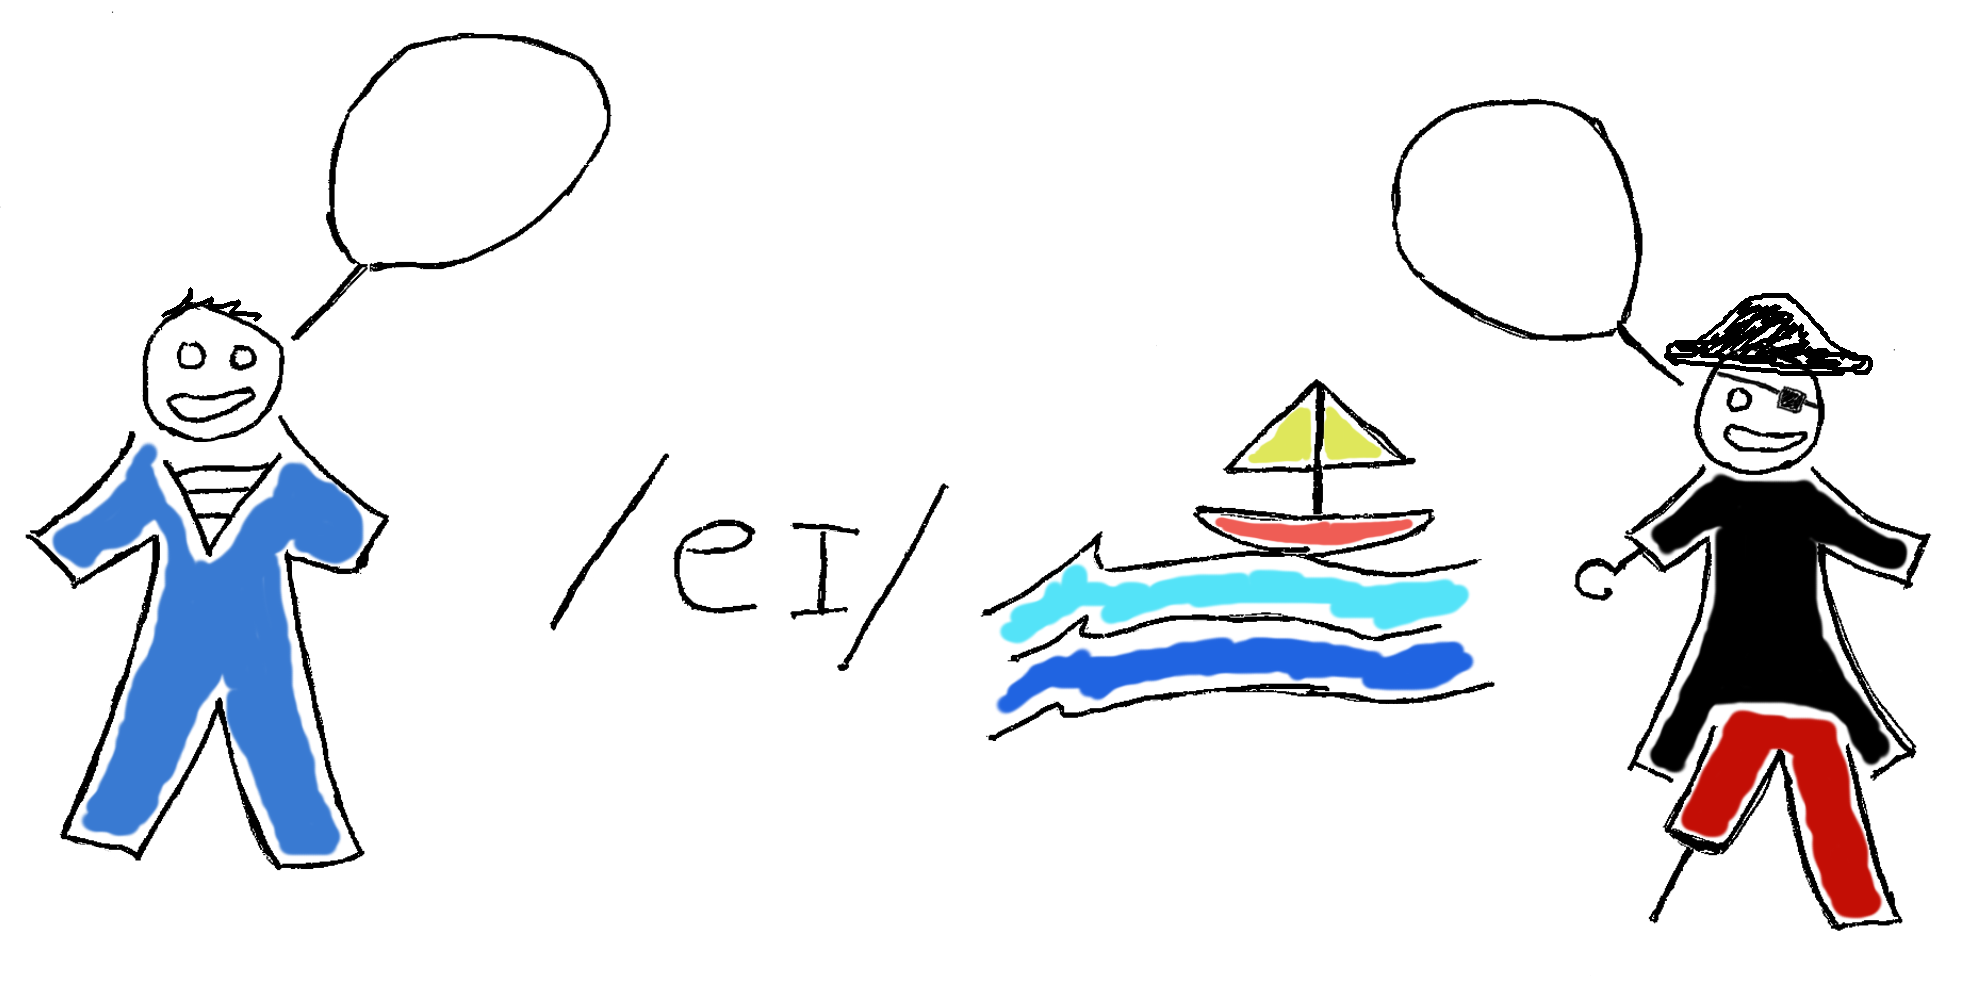
\includegraphics[scale=0.8]{iacr_coloured.png}
\end{turn}
\end{center}
\caption{A new flag for the IACR.\label{fig:iacr_flag}}
\end{figure}


\newcommand{\mybibtitle}[1]{\textsf{#1.}\hfil}
\newcommand{\mybibauth}[1]{#1.}
\newcommand{\mybibconf}[1]{\hspace*{\stretch{1}}\mbox{(#1)}}
\newcolumntype{z}{p{5em}}

\setcounter{section}{0}
\renewcommand\thesection{\Alph{section}}
\section[Mes publications]{My publications}

\subsection{Article de journal}

\noindent
\begin{tabularx}{\linewidth}{zX}
  \cite{asasajour} &
  \mybibtitle{Key-Recovery Attacks on ASASA}
  \mybibauth{B.~Minaud, P.~Derbez, P.-A.~Fouque, P.~Karpman}
  \mybibconf{En soumission, invité au J. Cryptology} \\
\end{tabularx}

\subsection{Articles de conférences}

\noindent
\begin{tabularx}{\linewidth}{zX}
  \cite{puppycipher} &
  \mybibtitle{Efficient and Provable White-Box Primitives}
  \mybibauth{P.-A.~Fouque, P.~Karpman, P.~Kirchner, B.~Minaud}
  \mybibconf{ASIACRYPT 2016} \\[2ex]
  \cite{DBLP:conf/eurocrypt/StevensKP16} &
  \mybibtitle{Freestart Collision for Full SHA-1}
  \mybibauth{M.~Stevens, P.~Karpman, T.~Peyrin}
  \mybibconf{EUROCRYPT 2016} \\[2ex]
  \cite{DBLP:conf/asiacrypt/MinaudDFK15} &
  \mybibtitle{Key-Recovery Attacks on ASASA}
  \mybibauth{B.~Minaud, P.~Derbez, P.-A.~Fouque, P.~Karpman}
  \mybibconf{ASIACRYPT 2015} \\[2ex]
  \cite{DBLP:conf/isw/Karpman15} &
  \mybibtitle{From Distinguishers to Key Recovery: Improved Related-Key Attacks on Even-Mansour}
  \mybibauth{P.~Karpman}
  \mybibconf{ISC 2015} \\[2ex]
  \cite{DBLP:conf/crypto/KarpmanPS15} &
  \mybibtitle{Practical Free-Start Collision Attacks on 76-step SHA-1}
  \mybibauth{P.~Karpman, T.~Peyrin, M.~Stevens}
  \mybibconf{CRYPTO 2015} \\[2ex]
  \cite{DBLP:conf/crypto/EspitauFK15} &
  \mybibtitle{Higher-Order Differential Meet-in-the-middle Preimage Attacks on SHA-1 and BLAKE}
  \mybibauth{T.~Espitau, P.-A.~Fouque, P.~Karpman}
  \mybibconf{CRYPTO 2015} \\[2ex]
  \cite{DBLP:conf/sacrypt/AugotFK14} &
  \mybibtitle{Diffusion Matrice from Algebraic-Geometry Codes with Efficient SIMD Implementation}
  \mybibauth{D.~Augot, P.-A.~Fouque, P.~Karpman}
  \mybibconf{SAC 2014} \\[2ex]
  \cite{DBLP:conf/ctrsa/0001KNWW14} &
  \mybibtitle{Analysis of BLAKE2}
  \mybibauth{J.~Guo, P.~Karpman, I. Nikolić, L. Wang, S. Wu}
  \mybibconf{CT-RSA 2014} \\[2ex]
  \cite{DBLP:conf/ima/FouqueK13} &
  \mybibtitle{Security Amplification against Meet-in-the-Middle Attacks Using Whitening}
  \mybibauth{P.-A.~Fouque, P.~Karpman}
  \mybibconf{IMACC 2013} \\
\end{tabularx}

\subsection{Prépublication}

\noindent
\begin{tabularx}{\linewidth}{zX}
  \cite{fly} &
  \mybibtitle{The \textsc{Littlun} S-box and the \textsc{Fly} block cipher}
  \mybibauth{P.~Karpman, B.~Grégoire}\\
\end{tabularx}

\section[Mes publications humoristiques]{My silly talks}

\subsection{Article de journal}

\noindent
\begin{tabularx}{\linewidth}{zX}
  & \mybibtitle{A new flag for the IACR}
  \mybibauth{P.~Karpman}
  \mybibconf{En soumission, invité au J. Craptology}\\
\end{tabularx}

\subsection{Présentations sans actes}

\noindent
\begin{tabularx}{\linewidth}{zX}
  &
  \mybibtitle{The Coffee Block Cipher Family --- A Snake Oil Candidate}
  \mybibauth{P.~Karpman}
  \mybibconf{ASIACRYPT 2014 (Rump session)}\\[2ex]
  &
  \mybibtitle{The \emph{Real} SHA-2,3,$\ldots$}
  \mybibauth{P.~Karpman}
  \mybibconf{CRYPTO 2015 (Rump session)}\\[2ex]
  &
  \mybibtitle{Breaking D.L. at Mont Saint-Michel}
  \mybibauth{P.~Karpman, B.~Minaud, A.~Wallet}
  \mybibconf{CHES 2015 (Rump session)}\\[2ex]
  &
  \mybibtitle{A new flag for the IACR}
  \mybibauth{P.~Karpman}
  \mybibconf{ASIACRYPT 2015 (Rump session)}\\
\end{tabularx}


\renewcommand\thesection{\arabic{section}}
